%\documentclass{revtex4-1}
\documentclass[10pt,a4paper,twocolumn,showkeys,showpacs,aps,groupedaddress]{revtex4-1}
\usepackage[utf8]{inputenc}
\usepackage[T1]{fontenc}
\usepackage{tikz}
% \usetikzlibrary{shapes,arrows,positioning}


\usepackage{lipsum}% for dummy text

\makeatletter
\renewcommand\@make@capt@title[2]{%
\@ifx@empty\float@link{\@firstofone}{\expandafter\href\expandafter{\float@link}}%
{\textbf{#1}}\@caption@fignum@sep#2\quad
}%
\makeatother

\begin{document}


\title{Aqui o título do paper}
\author{Salviano de A. Leão}\email{salviano@ufg.br}
\affiliation{Instituto de Física,\\
Universidade Federal de Goiás,\\
C.P.131, 74.001-970,\\
Goiânia (GO), Brasil}
\author{João Ninguém}\email{joao.niquem@gmail.com}
\affiliation{Instituto de Física de Lugar Nenhum,\\
Universidade Federal de Lugar Nenhum,\\
C.P.777, 99.999-999,\\
Lugar Nenhum (XX), Brasil}
%\date{Novembro de 2009}

\begin{abstract}
   Aqui deve vir o resumo do seu trabalho. Você deve explicar
   de forma sucinta o que você fez
\end{abstract}

\keywords{Palavra-chave01, Palavra-chave02, Palavra-chave03}

\maketitle

\lipsum[1]

\begin{figure}[ht]
\rule{5cm}{0.1cm}

\caption{\protect\lipsum[2]}
\label{fig:foo}
\end{figure}

\lipsum[3]

\begin{figure}[!htb]
\begin{center}
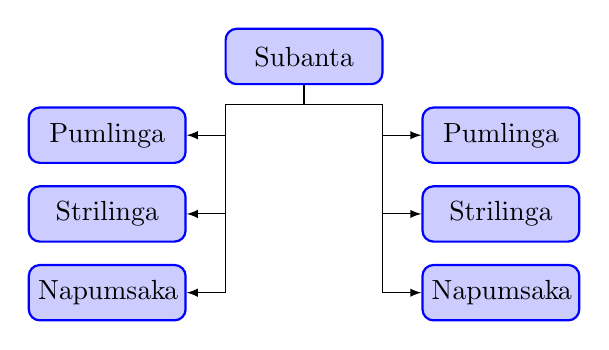
\begin{tikzpicture}
[auto,
 block/.style ={rectangle, draw=blue, thick, fill=blue!20, text width=5em,align=center, rounded corners, minimum height=2em},
 block1/.style ={rectangle, draw=blue, thick, fill=blue!20, text width=5em,align=center, rounded corners, minimum height=2em},
 line/.style ={draw, thick, -latex',shorten >=2pt},
 cloud/.style ={draw=red, thick, ellipse,fill=red!20,
 minimum height=1em}]
\draw (2.5,-2) node[block] (C) {Subanta};
\path (0,-3) node[block] (G){ Pumlinga}
      (0,-4) node[block] (H){ Strilinga}
      (0,-5) node[block] (I){ Napumsaka}
      (5,-3) node[block] (J){ Pumlinga}
      (5,-4) node[block] (K){ Strilinga}
      (5,-5) node[block] (L){ Napumsaka};
\draw (C.south) -- ++(0,-0.25) coordinate (linga);
\draw (linga) -- ++(-1,0) coordinate (ling);
\draw[-latex] (ling) |- (G.east);
\draw[-latex] (ling) |- (H.east);
\draw[-latex] (ling) |- (I.east);
\draw (linga) -- ++(1,0) coordinate (hling);
\draw[-latex] (hling) |- (J.west);
\draw[-latex] (hling) |- (K.west);
\draw[-latex] (hling) |- (L.west);
\end{tikzpicture}
\end{center}
\caption{Summary of Linga } \label{linga}
\end{figure}


\begin{tikzpicture}[sibling distance=10em, every 
   node/.style = {shape=rectangle, rounded corners, draw, align=center, top color=white, 
   bottom color=blue!20},
   line/.style ={draw, thick, -latex',shorten >=2pt}]
\end{tikzpicture}





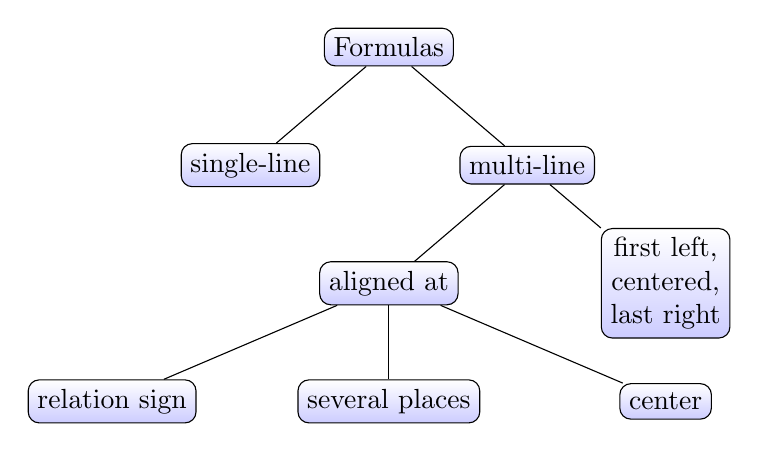
\begin{tikzpicture}[sibling distance=10em,
  every node/.style = {shape=rectangle, rounded corners,
    draw, align=center,
    top color=white, bottom color=blue!20}]
  \node {Formulas}
    child { node {single-line} }
    child { node {multi-line}
      child { node {aligned at}
        child { node {relation sign} }
        child { node {several places} }
        child { node {center} } }
      child { node {first left,\\centered,\\last right} } };
\end{tikzpicture}


\end{document}


